\chapter{技术综述}
为了满足彭庆福餐厅点单系统对于功能、可靠性、性能等方面的要求,在该系统的实现过程中,使用了Spring Cloud微服务部署架构、Spring Boot、Druid、Redis、React、Redux、Immutable、antd、Webpack、Kafka、微信支付宝支付、React封装的高德地图组件React-AMap等技术。本章将从技术原理、作用、优点等几个方面,对彭庆福餐厅点单系统中使用的技术进行简要的介绍。

\section{Spring Cloud微服务部署架构}
传统软件项目一般采用的都是单块架构,对于一个逻辑上会分为多层的系统,它会把经历开发、编译、测试、打包、部署后的代码运行到同一个进程内,不断扩大的业务规模和不断变更的业务逻辑会将单块架构的劣势愈演愈烈~\cite{sharma2017mastering}。不光是激增的模块、代码会使得项目变得冗余复杂,降低代码的灵活性、易用性和可维护性,各个功能模块往往也会依赖相同或是相关的内存、数据库等内容,如果某个资源模块出错有可能导致整个系统崩溃。

Spring Cloud微服务部署架构是一系列框架、组件的有序集合,它与Spring Boot相结合,大大降低了分布式系统对于日常开发的复杂度。它包括一连串功能完善的微服务组件,比如智能路由和服务发现、服务跟踪、消息总线、服务容错、断路器、负载均衡、服务配置等~\cite{zsf2019}。基于其各组件的完整架构图如下图
~\ref{fig_springCloudCH2}所示:
\begin{figure}[htbp!]
    \centering
    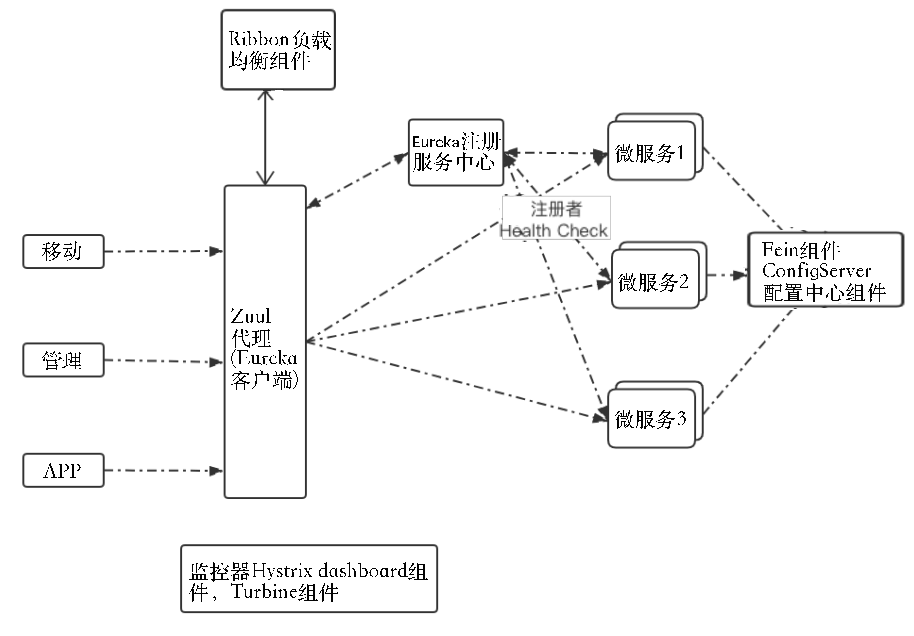
\includegraphics[width=5in]{FIGs/chapter2/springCloud.pdf}
    \caption{Spring Cloud架构图}\label{fig_springCloudCH2}
\end{figure}

Spring Cloud是一个框架,提供了在应用程序中使用云服务的工具。 当它与Eureka一起使用时,可以用作容器编排工具(提供用于大规模集成和管理容器的企业级框架的框架)~\cite{cosmina2017spring}。它为开发人员进行开发和部署微服务提供了友好的环境。其优点有:基于云原生的开发;基于微服务的架构;服务间通讯;遵循Spring Boot模型;与云无关。

\section{Spring Boot技术}
Spring Boot是一个Spring模块,向Spring框架提供RAD(快速应用程序开发)功能。它是一个在Spring框架顶部构建的项目,提供了一种简单、快速的方法来设置、配置和运行基于Web的应用程序。它简化了Spring的应用开发过程,节省了开发人员的时间,其核心思维是约定优于配置,尽量使其自发完成,简化系统开发。

如图
~\ref{fig_springBootCH2}
所示,Spring Boot是Spring框架(Spring Framework)和嵌入式服务器(Embedded Servers)的结合。在Spring Boot中,不需要XML配置(部署描述符)~\cite{sharma2019mastering}。它使用约定而不是配置软件设计范例,这意味着它减少了开发人员的工作量。
\begin{figure}[htbp!]
    \centering
    \includegraphics[width=5in]{FIGs/chapter2/springBoot.pdf}
    \caption{Spring Boot组成图}\label{fig_springBootCH2}
\end{figure}

Spring Boot使用了依赖注入方法,包含了强大的数据库事务管理功能,简化了与其他Java框架(如JPA/Hibernate ORM、Struts等)的集成,减少了应用程序的成本和开发时间~\cite{walls2016spring}。

Spring Boot的优点有很多:
\begin{itemize}
    \item 它创建可以使用Java -jar启动的独立Spring应用程序。
    \item 借助Tomcat、Jetty等不同的嵌入式HTTP服务器,可以轻松调试Web应用程序。
    \item 不需要部署WAR文件,能直接嵌入Tomcat中。
    \item 提供了自动配置的“starter”POMs(项目对象模型),来简化Maven配置。
    \item 提供了可用于生产的功能,例如指标、运行状况检查和外部化配置。
    \item 不需要XML配置。
    \item 提供了CLI工具,用于开发和测试Spring Boot应用程序。
    \item 提供了许多插件。
    \item 最大程度地减少了编写多个模板代码(该代码在几乎没有任何更改的情况下包含在许多地方)、XML配置和注释~\cite{antonov2018spring}。
\end{itemize}

\section{Druid数据库连接池}
Druid是一个高效的开源数据库连接池,可以聚合查找大量基于时序的数据,这里基于时序是指数据的实时性,从数据库实时获取数据放入Druid后,外部系统就可以立刻查到。

\begin{figure}[htbp!]
    \centering
    \includegraphics[width=5in]{FIGs/chapter2/druid.pdf}
    \caption{Druid工作流程图}\label{fig_druidCH2}
\end{figure}
如图
~\ref{fig_druidCH2}
官方提供的Druid工作流程图所示,Druid是由多种节点组成的分布式系统,每个节点按照职责划分成不同角色,包括如下五种类型。

\begin{itemize}
    \item Historical:这类节点用于存储和查询历史数据,需要从Deep Storage获取Segment,还需要响应Broker对于Segment的查询请求。此外,Historical还需要向Zookeeper声明自己的存在~\cite{yang2014druid}。
    \item Coordinator:这类节点用于检测Historical节点中数据的可用和冗余,通过Zookeeper来发现Historical节点。
    \item Broker:这类节点用于接收外部调用方的查询请求,然后转发到Historical和Realtime,并且还需要把结果Merge之后再返回给调用者,同样通过Zookeeper感知Historical和Realtime。
    \item Indexing Service:主要用于从Realtime获取实时数据或批量插入数据。
    \item Realtime:主要用于从数据库获取实时数据。
\end{itemize}

除了上述五种节点外,Druid还有三个外部依赖:用于管理各个Druid节点的Zookeeper集群;数据库存储实例,如MySQL等;用来做Deep Storage的HDFS~\cite{singh1990druid}。

\section{Redis}
Redis是一个完全开源免费的非关系型数据库(NoSQL),项目由VMWare赞助开发。它使用高效的C语言开发,基于键值对存储,支持网络交互,数据可以存储在内存也可以持久化存储~\cite{carlson2013redis}。在Redis中,Value支持如下几种数据类型:

\begin{itemize}
    \item String:字符串,是Redis中最基本的数据类型,也是任何存储系统都必备的数据类型。
    \item List:字符串列表,其中的数据是有序并允许重复的,底层实现是链表而不是数组。数据按照插入顺序排序,也可以在列表的头部、尾部或任意位置插入数据。
    \item Set:字符串集合,其中的数据是无序并且不允许重复的。基于哈希表实现,插入、删除、查找三种操作的时间复杂度均为常数级,效率较高。
    \item 	Sorted Set:有序字符串集合,基于Set之上添加了有序性,实现方法是为每个元素关联了一个浮点数类型的值,基于这个值来做数据的排序~\cite{lerner2010forge}。
    \item Hash:键值对哈希表,其中Key和Value都是String类型的,是从redis-2.0.0版本之后才支持的数据类型。
\end{itemize}

由于对内存中数据的读写速度远高于磁盘读写,因此Redis作为缓存使用时主要使用内存存储数据~\cite{macedo2011redis}。但Redis同样也支持数据持久化,主要有两种方式,分别是RDB(Redis DataBase)和AOF(Append Only File),两种方式可以同时使用。RDB简单来讲就是对Redis的内存数据生成一份快照并存储到磁盘等存储介质中,AOF则是将Redis执行过的所有写指令记录下来,数据恢复时只需要把这些指令按顺序执行即可。

此外,Redis具有原子性,即Redis的所有操作都是原子性的,执行结果只有成功和失败两种可能,同时也支持多个操作的事务管理~\cite{da2015redis}。这里的事务跟一般的数据库事务一样,是一种隔离操作,用于一次性按顺序执行多个指令。Redis事务同样具备原子性,如果Redis在某个事务执行过程中崩溃退出,导致该事务只执行了部分命令,那么Redis重启时会自动检测并移除部分执行的事务~\cite{nelson2016mastering}。

\section{前端技术}
该系统的前端开发主要使用React、Redux,其中React具有组件化开发、单项数据流的特性,使得其具有良好的灵活性、组件性、流动性、和隔离性,将一个页面划分成多组件进行开发,以此来独立开发功能之间相互独立的组件,并可以重复使用。同时使用了Immutable.js创建数据,减少系统内存消耗,界面的各类组件设计使用了蚂蚁金融开发的Ant Design设计体系的React UI组件库——antd,进行快速、美观、高效的前端界面开发。\\

\subsection{React和Redux}
React是一个声明式、组件化、高效灵活的用于构建UI用户界面的开源JavaScript库。使用React将创建交互式UI变得简单,为应用中的各类状态设计了简明视图,使得React能在数据发生变化时进行有效更新以及渲染组件,将代码变得可靠、清晰、方便调试~\cite{banks2017learning}。它创建了拥有独立状态的不同组件,再将这些简洁且独立的组件组合构成较为复杂的UI界面。

React组件可以接收各类数据使用render()方法进行界面渲染,通常存储为JSX类文件,被传入的外部数据通过this.props可以在组件内访问,此外组件还可以维护内部数据,通过this.state访问,通过this.setState()方法来更新,当组件内部数据发生改变时,组件会调用render()方法进行对应标记部分的重新渲染~\cite{sutcliffe1983antibodies}。

React有很多优点,它的组件化、模块化使得代码的复用性、可维护性非常高,使用虚拟DOM操作既解决了跨浏览器问题,提供了标准化API,又加快了渲染速度,提升Web性能,有序的单项数据流方便进行开发管理~\cite{chinnathambi2018learning}。然而,多个数据层与多个组件交互构成数据流时,随着数据规模的不断扩大,一些反响数据流就会变得十分复杂,从而产生许多无法估量的问题。这里引用了Redux,它是由Flux演变而来的,没有Flux的复杂性,变得简单、易上手,是JavaScript的状态容器,使得状态管理变得可预测~\cite{master2016}。

Redux具有三大特性:
\begin{itemize}
    \item 单一数据源:应用中的所有State都储存在一棵Object Tree中,且Object Tree只会在唯一的Store中存在。这就使得开发和调试变得简单,比较复杂的功能,例如撤销、重做也变得非常容易。
    \item State是只读的:改变State的方法只有一种——触发Action。Action是用来描述已经发生了的事件的一个普通对象,可以被序列化、存储、后期调试、日志打印或者测试时被回放。这样一来可以保证网络请求和界面视图都不可以直接修改State状态,如果想要修改则只能表达要修改的意图,然后由Redux集中处理,并且按照顺序逐个执行,不会出现竞态条件(Race Condition)。
    \item 使用纯函数执行修改:需要通过撰写Reducer来描述Action是如何改变State Tree状态树的。Reducer用于接收之前的State和Action,依次返回新的State,它是纯函数。用户可以编写很多可以独立操作State Tree不同功能部分的Reducer,控制其调用顺序、传入一些数据参数,也可以编写一些可复用的Reducer用于处理比如分页器等的通用任务~\cite{mardan2017react}。\\
\end{itemize}

\subsection{Immutable.js}
Immutable通俗来讲就是一个可以实现数据结构持久化的JavaScript库,它是一系列一经创建不能被改变的数据结构的集合,可以和Rudex对接良好。系统主要使用的几个持久化数据结构有:Set、List、Map,可以高效链接map、filter等方法。数据一旦创建无法更改,Immutable提供了一个可变API来产生新的更新数据,不去更新原有数据。这样可以简化应用程序的开发过程、减少内存消耗、使用简单的逻辑实现检测更新技术。\\

\subsection{antd}
antd是基于蚂蚁金融开发的Ant Design设计体系的一套React UI组件库,主要用于研发、设计企业级中后台的产品UI界面。它的出现可以提炼产品的视觉风格、交互语言,是开箱即用的质量比较高的React组件,与本系统的前端框架刚好吻合,支持多种语言、可以进行个性化主题定制,安装简单且容易上手。减少了人工设计基础组件的时间、成本浪费,可以有效提高系统的界面美观度和开发效率。\\

\subsection{React-AMap}
React-AMap是React封装的高德地图组件,可以比较简单、快速地将地图接入到项目中。本系统H5界面的外卖点单中用户地址的选择和Web界面的座位库平面视图均使用了该技术,主要用到的组件有Map、Marker,由于需求比较复杂、个性化,系统还根据高德地图原生的API自定义了组件MouseToolPlugin进行地图上图标的管理。

React-AMap组件拥有的属性,分为基本类型值和引用类型值,比如Map的属性zoom属于数字类型值,属性center属于引用类型值。定义React-AMap的引用类型属性,最好在React生命周期中的constructor和componentWillMount方法中实现,可以在组件中进行引用。在组件中,可以通过props访问到高德地图实例和其中的div容器类型,进而可以自定义地图组件和功能。React-AMap组件有一些已经存在的扩展组件,比如热力图组件(react-amap-plugin-heatmap)、定位组件(react-amap-plugin-geolocation)、可定义的AMapUI组件(react-amapui-wrapper)。\\

\subsection{Webpack}
Webpack一般用于前端的打包,它是一个JavaScript(JS)应用程序的高度可配置的静态模块打包工具,它通过递归构建包含应用开发程序所需要的各个模块的依赖关系图,接着将其打包成相应数量的bundle~\cite{subramanian2017modularization}。主要包括四个核心概念:entry、output、loader和plugins。其中entry用于指示使用哪个模块开始构建内部的依赖图,当找出入口起点直接和间接依赖的库或者模块时,将依赖处理并输出到bundles内,默认值是./src。output用于指定输出bundles的位置、如何命名,编译整个的程序结构到指定的输出路径文件夹,其默认值是./dist。由于Webpack本身只能理解JS,这就需要loader处理一些非JS文件,将其处理成Webpack可以进行打包的有效模块。打包优化、代码压缩、分离、去重、重新定义环境变量等内容都在plugins插件范围内,它依靠插件的接口功能可以处理很多复杂任务。

\section{Kafka消息系统}
Kafka是一个基于Zookeeper协调的分布式发布订阅消息系统,它支持分区、多副本、异步处理、高吞吐量、持久可靠、可扩展、负载均衡、容错性高、高并发,可以实时处理海量数据从而满足系统所需的各种场景~\cite{deleuze1986kafka}。主要是由Scala语言和Java语言编写,使用场景很多,可以用于收集各种服务log日志;跟踪用户活动,做一些监控、离线分析、挖掘;高解耦可用作消息系统;收集数据并生产各种操作的反馈,记录运营监控数据,用于运营指标;可以进行一些比如Spark Steaming等的流式处理;事件源~\cite{kafka1979basic}。

Kafka具有四个比较核心的API~\cite{kreps2011kafka}:
\begin{itemize}
    \item Producer API可以让应用程序的记录流发布到若干个Kafka主题。
    \item Consumer API可以让应用程序订阅若干Kafka主题,处理生成的记录流。
    \item Streams API可以让应用程序作为流处理器,使用若干主题的输入流来生成若干输出主题的输出流,从而有效可靠地把输入流转换成为输出流。
    \item Connector API可以构建、运行可重用生产者或者使用者,它们将Kafka主题链接到已有的应用程序、数据系统。
\end{itemize}

\section{微信支付宝支付}
\subsection{微信支付}
微信支付参照其开发文档,支付模式一共有六种,分别是付款码支付、Native支付、JSAPI支付、APP支付、H5支付、小程序支付~\cite{xu2017study}。本系统是嵌入在微信、浏览器中的H5界面和Web界面,用到了以下三种支付模式:
\begin{itemize}
    \item Native支付:系统的Web网页端按照微信给的支付协议生成商家的支付二维码,用户打开微信“扫一扫”,扫码完成支付。该模式适用场景有:PC端网站支付、实体商店单品支付、订单扫码支付、媒体支付、广告支付等。
    \item JSAPI支付:用户在微信中打开商家的H5页面,本系统的H5界面嵌入在微信公众号内,商家在该页面通过后端调用微信支付所提供的JSAPI支付接口,回调微信支付模块以此完成支付功能。该模式适用场景有:用户从微信点击进入商家公众号,从某商家主页完成支付;用户在聊天界面、朋友圈等点击商家链接,打开页面完成支付;用户扫描由商家页面转换成的二维码,从微信浏览器中进入该商家页面进行支付操作。
    \item 	H5支付:用手机、平板等移动设备通过浏览器进入商家页面,唤起微信支付进行支付。
\end{itemize}

本系统的顾客点单平台中,嵌入在微信公众号内的H5界面,需要在微信平台内进行支付,支付方式只能用微信支付。
首先需要登录公众号进行JS接口安全域名的填写,并获取openid,它是商家在微信公众号appid下的唯一用户标识(与appid一一对应),可以永久标记用户,也是使用JSAPI支付必须要传的一个参数。
用户新建一个授权url页面,当授权成功会根据用户设定的(redirect uri)重定向地址
跳转到相应地址,并得到授权返回的code,将该code码作为参数调用后端接口,返回openid。
在微信公众号内,需要添加支付页面的地址,并将其作为参数调用后端接口,返回值可以配置wx.config。获得返回值后,再通过wx.ready调用wx.chooseWXPay进行微信支付即可支付成功。\\

\subsection{支付宝支付}
支付宝的支付功能比微信支付简单一些,它能在非微信平台内调用。支付宝支付需要有支付宝开放平台的账号,在该网站内创建一个应用,填写相关信息,审核通过后即可配置沙箱环境。由于支付涉及到金钱安全问题,支付宝提供了一种模拟支付环境——蚂蚁沙箱环境,用来帮助开发者对功能接口进行开发和联调。

\section{本章小结}
本章主要从定义、工作原理、架构、特性等几个方面,介绍了彭庆福餐厅点单系统开发过程中用到的相关开发框架和技术。整个系统采用Spring Cloud微服务部署架构进行搭建,与Web服务相关的接口按照REST风格进行设计。其中,后端技术使用了Spring Boot,数据库用到了MySQL、Druid、Redis,前端技术使用了antd、React、Redux、微信支付宝支付以及高德地图组件React-AMap、Immutable、Webpack,还介绍了Kafka消息系统。
